\documentclass[11pt,letterpaper]{article}
\usepackage[margin=.81in,top=.79in,bottom=.77in,headheight=14pt,headsep=13pt]{geometry}
\usepackage{amsmath,amssymb,booktabs,xcolor,array,tikz,hyperref,fancyhdr}
\usetikzlibrary{arrows.meta,positioning}
\definecolor{navy}{HTML}{17354A}\definecolor{teal}{HTML}{116658}
\definecolor{dim}{HTML}{456272}\definecolor{wash}{HTML}{EAF4F1}\definecolor{brick}{HTML}{9C462F}
\hypersetup{colorlinks=true,urlcolor=teal,linkcolor=teal,pdftitle={Single-tour routing and Hamiltonian count bits},pdfauthor={Research note prepared for Dominic Dabish}}
\pagestyle{fancy}\fancyhf{}\fancyhead[L]{\small\sffamily\color{teal}SINGLE-TOUR ROUTING}
\fancyhead[R]{\small\sffamily\color{dim}COMPLEXITY THEORY}
\fancyfoot[L]{\footnotesize\sffamily\color{dim}Working manuscript for Dominic Dabish \enspace / \enspace 21 November 2026}
\fancyfoot[R]{\small\sffamily\color{navy}\thepage}\renewcommand{\headrulewidth}{.35pt}
\setlength{\parindent}{0pt}\setlength{\parskip}{5pt}\setlength{\emergencystretch}{1em}
\setlength{\abovedisplayskip}{5pt}\setlength{\belowdisplayskip}{5pt}
\newcommand{\bnd}[1]{\par\smallskip\noindent\colorbox{wash}{\parbox{\dimexpr\linewidth-2\fboxsep\relax}{\vspace{3pt}#1\vspace{3pt}}}\par\smallskip}
\newcommand{\subh}[1]{\par\smallskip{\large\bfseries\color{teal}#1}\par\nobreak}
\newcommand{\pg}[2]{\newpage\phantomsection\pdfbookmark[1]{#1}{#2}{\LARGE\bfseries\color{navy}#1\par}\smallskip}
\newcommand{\lab}[1]{\textbf{\color{navy}#1}\enspace}
\newcommand{\pf}{\operatorname{Pf}}\newcommand{\hc}{\operatorname{hc}}\newcommand{\PPa}{\mathord{\oplus}\mathrm P}
\newcommand{\GF}{\mathbb F_2}\newcommand{\sat}{\operatorname{\#SAT}}
\newcommand{\citeurl}[2]{\href{#1}{#2}}
\begin{document}
\phantomsection\pdfbookmark[1]{Results and pathway}{first}
{\sffamily\small\color{dim} RESEARCH NOTE \hfill ALGORITHMS, COUNTING AND SUDOKU}\\[8pt]
{\fontsize{25}{29}\selectfont\bfseries\color{navy}Single-tour routing and\\Hamiltonian count bits\par}
\medskip
A switch exchanges two lanes when its control bit is on. Run a sequence of switches, connect each output back to the correspondingly numbered input, and trace the resulting loops. Can the controls be set so that there is just one loop through every lane? A control can govern several switches, and fixed swaps can be inserted anywhere. The number of uses counts individual controlled transpositions.

\subh{A sharp threshold for the decision problem}
\begin{center}
\renewcommand{\arraystretch}{1.26}\begin{tabular}{@{}lccc@{}}
\toprule
Maximum uses per bit & One tour exists & Parity of settings giving one tour & Exact count\\
\midrule
One   & P & P & FP\\
Two   & P & P & \#P-complete$^*$\\
Three & NP-complete & $\PPa$-complete & \#P-complete\\
\bottomrule
\end{tabular}
\end{center}
{\small $^*$The two-use counting result uses the usual polynomial-time counting reductions for the permanent. The three-use reductions preserve the number of solutions. Each setting of the occurring control bits counts once. FP means the integer answer is computable in deterministic polynomial time.}

\subh{The route from Sudoku}
\begin{center}
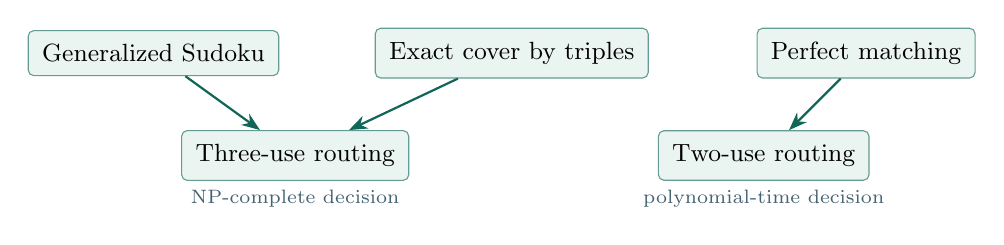
\begin{tikzpicture}[>=Stealth,box/.style={draw=teal!65,fill=wash,rounded corners=2pt,inner sep=5pt,align=center,font=\small},ar/.style={->,teal,thick}]
\node[box] (s) at (-4.55,1) {Generalized Sudoku};
\node[box] (x) at (0,1) {Exact cover by triples};
\node[box] (m) at (4.5,1) {Perfect matching};
\node[box] (r) at (-2.75,-.3) {Three-use routing};
\node[box] (t) at (3.2,-.3) {Two-use routing};
\draw[ar] (s)--(r);\draw[ar] (x)--(r);\draw[ar] (m)--(t);
\node[font=\scriptsize,text=dim] at (-2.75,-.85) {NP-complete decision};
\node[font=\scriptsize,text=dim] at (3.2,-.85) {polynomial-time decision};
\end{tikzpicture}
\end{center}
The obvious strategy of replacing a three-way copy of a bit with a network of two-use controls fails for a structural reason. Page 5 proves that every such network with one use per exposed bit obeys an exchange law. The relation accepting precisely $000$ and $111$ violates it.

\subh{A separate bit of graph structure}
A cubic bipartite graph has an even number of undirected Hamiltonian cycles. Pages 6--7 construct one such graph from a formula so that its \emph{second} binary digit is the parity of the satisfying-assignment count. Page 8 gives a different graph and a specified higher digit that decides satisfiability deterministically. Computing that digit on arbitrary outputs is the outstanding step toward P versus NP.

\pg{One use and the reference Euler tour}{one}
\lab{The exact one-use count.} For width $d$, write $P(b)$ for the resulting $d\times d$ permutation matrix. Fix a lane $r$ and delete its row and column from $I-P(b)$. Its determinant is one if $P(b)$ is a single cycle and zero otherwise. Indeed, every cycle excluding $r$ contributes a singular block. For a single cycle the remaining permutation arcs form a path and can be put in triangular order with unit diagonal. The empty determinant is one.

If an independent control governs one swap $S$, replace its matrix by $(I+S)/2$. Write $\bar P$ for the product of the resulting matrices and the fixed permutations in their original order. With $m$ independent controls,
\[
N_{\mathrm{tour}}=2^m\det\bigl((I-\bar P)_{\widehat r,\widehat r}\bigr).
\]
To prove the formula, interpolate one factor by $I+t(S-I)$. The difference $S-I$ has rank one. Multiplication on both sides by the other factors and deletion of one row and column preserve the rank bound. A determinant under a rank-one update is affine in $t$ by column multilinearity. This remains true after averaging any of the other independent factors. Substituting $t=1/2$ everywhere therefore gives the average of the vertex values on the Boolean cube. Rational elimination has polynomial bit complexity since the scaled entries have $O(m)$ bits and minors have polynomial bit length.

\subh{Turn the program into a circuit partition}
Collapse the wires and all fixed swaps between controlled switches. Each remaining switch is a vertex with two incoming and two outgoing wire ends. Its straight and crossed settings are the two directed transitions. The number of directed circuits equals the number of cycles of the resulting permutation on lanes. Wire-only components can be handled immediately. A wire-only component together with another component prevents a single tour. With no switches, trace the fixed permutation directly.

Ignore repeated-control constraints temporarily. A connected directed graph with balanced indegrees and outdegrees has an Euler circuit $C$. One can build it by joining the circuits of any initial transition system at common vertices. If the underlying transition graph is disconnected, one circuit is impossible. Each switch occurs twice on $C$. Form its \emph{interlacement matrix} $A$ over $\GF$ with zero diagonal. Entry $A_{ij}=1$ exactly when the occurrences of $i$ and $j$ alternate along $C$.

\bnd{\textbf{Cohn--Lempel circuit-nullity equality.} If $T$ lists the transitions flipped from $C$, the resulting circuit count is $1+\operatorname{nullity}_{\GF} A[T]$. Consequently the settings yielding one circuit are precisely the nonsingular principal submatrices. The reference circuit fixes the bit convention at each switch.}

A bit with two occurrences requires the two relative flips to be equal or opposite, according to these conventions. A negated control simply changes the convention at its switch. All later computations use these relative flips. The circuit-nullity equality and its graph formulation are classical [1].

\pg{Two uses, decision and parity}{two}
\lab{Deterministic decision.} The subsets $T$ with $A[T]$ nonsingular form a binary linear delta-matroid $D_A$. There is also a small linear representation of the permitted even-cardinality choices of flips. Use a separate $2\times2$ alternating block with off-diagonal entries one for every pair. Its feasible choices are both or neither. For an opposite pair, toggle one designated coordinate in every feasible set. This operation is a \emph{twist}.

On the singleton occurrences put the adjacency matrix of a complete graph. Its principal submatrix on $k$ vertices equals $I+J$ over $\GF$ and is nonsingular exactly for even $k$. If the number of opposite pairs is odd, the singleton selection must be odd. Twist one singleton to permit all such choices. If none exists in that case, return no. The resulting twisted direct sum $D_B$ represents all and only the permitted even subsets. An accepting assignment exists exactly when $D_A,D_B$ have a common feasible set.

Take their direct sum on two copies of the ground set and pair each index with its twin. A feasible set with zero broken pairs selects the same indices in both copies. The deterministic linear delta-matroid parity algorithm of Geelen, Iwata and Murota finds the minimum number of broken pairs in polynomial time [2]. The companion implementation starts at the twist in the direct sum, augments across two broken pairs at a time, and returns an actual winning control setting or a definitive no answer. Reading the common subset in either copy recovers the setting through the reference conventions.

\subh{One binary determinant gives the parity}
Start with $A$. For an equal pair $i,j$, add a formal edge $z_{ij}$ to entry $ij$ and its transpose. For an opposite pair add a new vertex and join it by separate formal edges to $i$ and $j$. Let $N$ be the current matrix order. If $N$ is odd, add one further vertex. Add separate formal edges in a clique on all singleton occurrences and this last vertex if present. All new weights are distinct variables. Call the resulting alternating matrix $M$.

Expand its Pfaffian over matchings. Choosing the formal edges first leaves the principal submatrix $A[T]$. Equal pairs have either both endpoints left or both removed. An opposite pair has one left. Every admissible $T$ of even size leaves an even number $k$ of excluded singleton and extra vertices for the clique. They can be paired in $(k-1)!!$ ways, an odd number, with one way for $k=0$. Thus, on setting every $z$ to one, the Pfaffian gives the parity of the winning settings. In $\GF$, $\det M=(\pf M)^2=\pf M$.

Keeping the variables formal also gives a shorter randomized existence implementation. Each particular choice of formal matching edges has its own monomial. Its coefficient is $\pf A[T]$. Hence the polynomial is nonzero exactly when a winning setting exists. Its degree is at most half the order of $M$. Choosing weights independently in a field of size greater than twice that order has false-negative probability below $1/4$ per trial. A positive answer is conclusive. The software includes this optional independent test, the exact binary parity calculation, and the deterministic augmenting-path solver above.

\pg{Why triples already encode SAT}{cover}
For each required element build two directed rings with corresponding positions $a_1,\ldots,a_d$ and $b_1,\ldots,b_d$. Traverse the $a$ ring forward and the $b$ ring backward. At position $i$, candidate $i$ can switch the two successors. The fixed permutation is the product of the two counter-rotating cycles. The controlled transpositions $(a_i\,b_i)$ are disjoint within this block.

\begin{center}
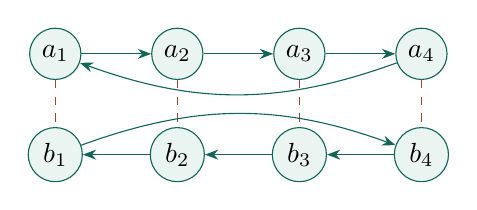
\begin{tikzpicture}[x=1.55cm,y=.64cm,>=Stealth,point/.style={circle,draw=teal,fill=wash,inner sep=2.6pt}]
\foreach \i in {1,2,3,4}{\node[point] (a\i) at (\i,1) {$a_\i$};\node[point] (b\i) at (\i,-1) {$b_\i$};\draw[brick,dashed] (a\i)--(b\i);}
\foreach \i/\j in {1/2,2/3,3/4}{\draw[->,teal] (a\i)--(a\j);\draw[->,teal] (b\j)--(b\i);}
\draw[->,teal] (a4) to[bend right=-20] (a1);
\draw[->,teal] (b1) to[bend right=-20] (b4);
\end{tikzpicture}\\[-1pt]
{\small\color{dim}Dashed pairs mark controlled swaps. Each swap exchanges outgoing successors.}
\end{center}

\lab{Exact-one lemma.} If no position is selected there are two cycles. If $k\ge1$ positions are selected there are exactly $k$ cycles. From each selected position follow the forward interval to the next selected position, then the backward interval on the opposite ring. This closes one circuit for each cyclic interval between consecutive selections. For $k=1$ the interval wraps all the way around both rings.

For each element choose one anchor on its $a$ ring. After all local operations add a fixed swap from the first anchor to each other anchor. Each such swap merges the distinguished circuits of two previously separate blocks. The total is $1+\sum_v(c_v-1)$ circuits, where $c_v$ is the local count. Therefore a global tour exists for exactly the selections covering every element once. An uncovered element with zero incident candidates is an immediate no instance.

\lab{Two uses.} Take elements to be vertices of a bipartite graph and candidates to be its edges. Each bit occurs twice. The winning settings are exactly its perfect matchings. Their count is the permanent of its bipartite adjacency matrix. Valiant's theorem gives \#P-hardness under polynomial-time counting reductions [3]. Guessing one setting gives membership.

\lab{Three uses.} Take candidates to be the triples of Exact Cover by 3-Sets. Every bit appears exactly three times. Each exact cover gives one winning setting and conversely. Hunt et al.\ provide a parsimonious SAT-to-X3C chain [4]. Decision is consequently NP-complete, parity is $\PPa$-complete and exact counting is \#P-complete under parsimonious reductions. This proof uses global wiring and a single tour as the acceptance condition.

\pg{Sudoku and the limit of copying a bit}{copy}
A candidate digit uses four exact-cover constraints. They require the cell, row--digit, column--digit and box--digit to be covered once. Discard candidates contradicted by clues in their cell. Give the first two incidences one bit $p$ and the last two another bit $q$. At the end add a fresh lane $z$ and, on the pair consisting of $z$ and a fixed old lane, apply a swap under $p$, a swap under $q$, and a fixed swap. If $p=q$, the net swap inserts $z$ in the old circuit. If $p\ne q$, lane $z$ remains a separate fixed point. Distinct checks use distinct fresh lanes. Each bit now has exactly three uses. The association between Sudoku completions and one-tour settings is bijective.

For an empty order-$N$ board with square boxes, this construction has $2N^3$ controls, $6N^3$ controlled swaps and $9N^3$ lanes. At $N=9$ the figures are 1,458, 4,374 and 6,561 respectively. Complexity statements concern growing $N$.

\subh{Can another copy step get from three uses down to two?}
Suppose three exposed bits each occur once inside a proposed simulator. Other bits may occur once or twice, in arbitrary numbers. For exposed settings, accept if the remaining bits can be set to obtain one tour. Every nonempty family of accepted exposed subsets $\mathcal F$ obeys \emph{symmetric exchange}. For $X,Y\in\mathcal F$ and $i\in X\triangle Y$ there is $j\in X\triangle Y$ such that $X\triangle\{i,j\}\in\mathcal F$. Choosing $j=i$ toggles just $i$.

\lab{Proof.} Use the Euler reference and put an independent indeterminate on each formal edge for paired internal controls as on page 3. Treat all singleton controls, exposed or internal, as boundary coordinates for now. Let $I$ contain both occurrences of each internal pair and every added opposite-pair vertex. For a chosen singleton subset $U$, the formal alternating submatrix $M[I\cup U]$ is nonsingular over $\GF(\mathbf z)$ exactly when some legal internal pair choices complete those flips. This follows by the Pfaffian monomial argument. No singleton clique is added at this stage.

Nonsingular principal submatrices of an alternating matrix obey symmetric exchange [2]. Restrict to feasible sets containing $I$. An exchange between two such sets touches only their difference, so it retains $I$. Delete $I$ from these sets. Project away the free internal singletons. For two feasible projected sets take any feasible lifts. If the exchange partner in the lifts is hidden, the projected move toggles only $i$. An exposed partner gives an ordinary two-coordinate move. Flipping reference conventions by a fixed set preserves the law.

\bnd{The relation $\{000,111\}$ fails the law. Starting at $000$, exchanging one or two coordinates cannot reach an accepted nonzero setting. Hence no simulator of the specified form, of any size, implements equality on three exposed bits.}

This rules out a local copy strategy with independently exposed ports. The three-use decision problem still admits arbitrary global algorithms as a mathematical possibility. A deterministic polynomial-time one would decide SAT.

\pg{The second bit of a Hamiltonian count}{mirror}
Let $\hc(G)$ count Hamiltonian cycles once each as undirected edge sets. Thomason's proof records that every edge of a cubic graph lies on an even number of Hamiltonian cycles, and that the \emph{total} is even in a cubic bipartite graph [5]. We derive the following stronger computational distinction.
\bnd{\textbf{Theorem.} On connected simple cubic bipartite graphs, testing $\hc(G)\equiv2\pmod4$ is $\PPa$-complete under deterministic polynomial-time many-one reductions. Hardness holds even if one Hamiltonian cycle is supplied.}

Start with a connected, simple, bipartite source $H$ with all degrees two or three and an edge $e=uv$ at a degree-two vertex $u$. Hamiltonicity of maximum-degree-three grid graphs is parsimoniously hard by the MIT Hardness Group et al.\ [6]. Such a finite grid has a vertex of degree at most two by an extreme-corner argument. Disconnection, degree below two or a bridge probe gives zero cycles and can be detected directly. A fixed cubic bipartite graph with zero cycles serves as an even output (see page 8). We handle the other cases below.

Delete $e$ and add a new leaf $t$ at $v$. In this sheet the leaves $s=u,t$ are on the same side. Its Hamiltonian $s$--$t$ paths correspond bijectively to cycles of $H$. Take two copies with opposite bipartitions. Add one edge between copies of every degree-two ordinary vertex and of each leaf. These edges are called rungs. All degrees are now three except the four terminal vertices $s_0,t_0,s_1,t_1$ of degree two. Denote the resulting fragment by $B$.

\lab{Seven boundary counts.} A tour traversing a balanced four-terminal fragment uses two or four external edges. With two, it is a spanning path joining a terminal on side 0 to one on side 1. Denote the four counts by $h_{00},h_{01},h_{10},h_{11}$, with $s$ indexed 0 and $t$ indexed 1 within each sheet. With four, two disjoint spanning paths pair the endpoints. Write $P$ for $s_0s_1,t_0t_1$, $Q$ for $s_0t_1,t_0s_1$, and $D$ for $s_0t_0,s_1t_1$. Extra internal cycles are excluded in all seven counts.

Sheet exchange interchanges the two paths of any fixed $D$ cover. Such a cover uses no rung, because a rung is fixed as an edge and the paths are disjoint. Thus each sheet carries one Hamiltonian path and the two paths are copies of one another. In a fixed $Q$ cover the paths likewise interchange, yet each must cross sheets, an impossibility without a rung. Writing $f=\hc(H)\bmod2$ gives $D\equiv f$ and $Q\equiv0$ modulo two.

\lab{Completing the signature.} Cap the fragment by two adjacent vertices, one joined to both terminals on each side, with bipartitions chosen consistently. Tours using the central cap edge contribute $\sum h_{ij}$, which is even by edge parity. Total parity gives $P+Q$ even. Edge parity at each spoke now makes each row and column sum of $(h_{ij})$ even. Finally close $B$ by adding just the two edges of the $Q$ pairing, both new. Tours through $s_0t_1$ number $h_{01}+P+D$, an even integer. Hence the seven counts in the displayed order have parity vector $f(1,1,1,1,0,0,1)$.

\pg{A single graph extracts the hard bit}{skeleton}
The adjacent pair of vertices used as a cap on page 6 is itself a four-terminal fragment. When two outside edges are used it has one spanning path for every opposite-side choice. With four edges used, the two vertices separately join their incident ends, yielding only pairing $D$. Its exact signature is therefore
\[
                       d=(1,1,1,1,0,0,1)^\mathsf T.
\]

Take $K_{3,3}$ with left vertices $L_0,L_1,L_2$ and right vertices $R_0,R_1,R_2$. Replace the adjacent pair $L_0,R_0$ by $B$. Replace $L_1,R_1$ by an identical copy with the port correspondence transported by the simultaneous interchange of 0 and 1. For an explicit convention, at $L_i$ attach the edge to $R_{1-i}$ to port $s_0$ and the edge to $R_2$ to $t_0$. At $R_i$ attach the edge to $L_{1-i}$ to $s_1$ and the edge to $L_2$ to $t_1$. The two remaining vertices and their connecting edge stay. The output is connected, simple, cubic and bipartite. For an $n$-vertex source it has $4n+6$ vertices.

Fix the spanning path state in each fragment. Which outside edges complete those states to a single tour depends only on the two boundary states. Thus the total for two copies with signature $v$ is $v^\mathsf T Mv$ for a fixed nonnegative integer matrix $M$. An outside edge directly linking the fragments is an ordinary edge in this count. Swapping the two fragments proves $M=M^\mathsf T$. Substitution of the two original adjacent pairs restores $K_{3,3}$ and gives $d^\mathsf TMd=6$. Indeed the complement of each of its six perfect matchings is a Hamiltonian cycle.

Page 6 gives $v=fd+2z$ for some integer vector $z$. Symmetry gives the integer identity
\[
 v^\mathsf TMv=6f^2+4f\,d^\mathsf TMz+4z^\mathsf TMz
                 \equiv 2f\pmod4.
\]
This proves a one-instance reduction. Membership in $\PPa$ follows by guessing an unordered pair of distinct tours in canonical edge-set order. For even $h$, $\binom h2\bmod2$ is its second binary digit.

\subh{Supplied tours and higher fixed digits}
For a formula $F$, a selector can choose either a model of $F$ with an auxiliary bit fixed, or the all-zero original input with that bit free. The padded formula has $\sat(F)+2$ models, including two known ones. The published source reduction translates a supplied model into a tour of $H$. Use its $s$--$t$ path in each sheet of each fragment, realizing state $D$. The six outer edges from the complement of the diagonal perfect matching in $K_{3,3}$ join these paths into a public tour.

Replace one vertex in a cubic bipartite graph by $K_{2,3}$, attaching its three degree-two vertices to the old neighbors. Every tour uses two boundary edges and there are exactly two spanning internal paths between the chosen ports. This doubles the entire count. Repeating $j-1$ times carries hardness to any fixed bit $j\ge1$, with the units bit numbered zero. Membership follows from $\binom h{2^j}\bmod2=\operatorname{bit}_j(h)$, by the binary factorization of $(1+x)^h$ over $\GF$. The certificate lists a constant number of tours for fixed $j$. The construction makes no planarity promise.

\pg{A specified digit decides satisfiability}{shift}
For $F$ on $n\ge1$ bits, use a selector $y$. If $y=1$, require $F(x)$. If $y=0$, require at least one $x_i=1$. Add the clause $y\lor x_1\lor\cdots\lor x_n$ and guard each original clause $C$ by $\neg y\lor C$. The resulting number of models is
\[
                        h=2^n-1+\sat(F).
\]
Its bit $n$ is set exactly when $F$ is satisfiable. A model is known in advance. The parsimonious grid theorem gives a graph $H$ with exactly $h$ tours. We give an exact regularization to preserve these digits up to an explicitly known shift.

\lab{Construct a path through every added scaffold vertex.} The padded source has a tour, so it is balanced bipartite, connected and of minimum degree two. Choose a forced edge at a degree-two vertex and subdivide it four times. The tour count is unchanged. The number $d$ of degree-two vertices is now even and at least six. There are equally many in both sides by the degree sums. Put $d$ new vertices on a ring, each paired by a rung to a distinct degree-two source vertex, ordering them so their colors alternate and rungs cross the bipartition. This makes a cubic bipartite graph.

Cut one of the new interior source path edges $ab$ and a ring edge whose ends are neither rung mate of $a,b$. At most four ring edges meet those mates. Cross-connect $a,b$ to the two exposed ring vertices preserving bipartition. Mark the ring path of $d-1$ edges and these two connectors. A tour containing all $d+1$ marks must traverse the entire ring path and cannot take any rung. Contracting this detour to $ab$ recovers precisely one source tour. Every source tour lifts uniquely with the marks.

\lab{Forcing a marked edge with constant multiplicity.} Join two copies of $K_{3,3}$ by deleting one edge in each and reconnecting their four ends by two bipartition-preserving cross edges. Every tour uses both edges of this two-edge cut. Delete a vertex incident with one cut edge. The resulting 11-vertex fragment has three ports. A spanning path between the two ordinary ports would give a tour omitting that cut edge, so the count is zero. From the distinguished port to either ordinary port the count is $2\cdot4=8$. In the first $K_{3,3}$ a specified incident pair lies on two tours, and in the second the removed edge lies on four.

Replace one endpoint of each marked edge by this fragment, assigning the marked edge to the distinguished port. At every three-edge boundary a spanning tour must use two edges and a single spanning path. Each substitution therefore gives eight lifts to every tour containing the mark and none to any other. Original edge identities persist as external incidences, so consecutive substitutions may share endpoints. The final cubic bipartite $G$ satisfies
\[
       \hc(G)=2^{3(d+1)}h,\qquad
       \operatorname{bit}_{3(d+1)+n}\hc(G)=\mathbf1_{\sat(F)>0}.
\]
The graph size and index are polynomial, and the construction can lift the known tour. For generic sources, easily detected zero cases can return a fixed zero-tour graph. Attach three $K_{3,3}$-minus-edge blocks between two new vertices using all six exposed ends. Removing the two new vertices leaves three components, precluding a tour. The package also implements a shorter specialized regularization for sources with adjacent pairs of wire vertices. Replacing each pair by $K_{3,3}$ minus one edge gives exactly four lifts per wire.

\pg{Checks, counterexamples and the open step}{checks}
\lab{The deterministic parameter bound.} If $k$ bits in an arbitrary program occur at least three times, fix those $k$ bits in all $2^k$ ways. Fold their gates into the fixed permutations and run the two-use decision algorithm on each residual program. This gives $2^k\operatorname{poly}(L)$ time for an explicitly encoded program of length and width totaling $L$. The three-use hardness construction lets $k$ grow with the input. The earlier problem of extending four prescribed edge colors with connected unpinned remainder also remains unresolved here.

\lab{A failed determinant shortcut.} In four lanes let one bit choose between $P_0=(0\,1)(2\,3)$ and $P_1=(0\,3)(1\,2)$. Their quotient is a product of two disjoint swaps, so this needs one control used twice. Each permutation has two circuits and each individual cofactor is zero. Their average matrix is the random-walk matrix on a four-cycle. Deleting row and column 3 from $I-(P_0+P_1)/2$ gives a cofactor of $1/2$ (also $4/2^3$ from its four spanning trees). Averaging these coupled gates as a single matrix would return a positive answer on an infeasible instance.

\lab{Small graph counts.} The verifier counted complete undirected tours as edge sets, independently of the seven-state formula. The probe is a degree-two edge in each source.
\begin{center}
\begin{tabular}{@{}lrrrc@{}}
\toprule
Source $H$ & $\hc(H)$ & Target vertices & $\hc(G)$ & $\hc(G)\bmod4$\\
\midrule
Four-cycle & 1 & 22 & 14 & 2\\
$K_{3,3}$ with one edge removed & 2 & 30 & 160 & 0\\
$K_{2,3}$ & 0 & 26 & 48 & 0\\
\bottomrule
\end{tabular}
\end{center}

\lab{Reproducible verification.} The bundle exercises 506 two-use programs and 10,694 assignments, including 192 feasible programs with an even winning count. The deterministic two-use solver also passed 4,182 independent matrix/twist comparisons. The bundle compares 250 one-use exact counts with enumeration, checks projected exchange on 200 small programs, compares 265 bipartite perfect-matching counts, and verifies 4,247 copy settings on 150 programs. The Sudoku tests trace all 288 completed $4\times4$ boards and reject one corrupted copy per board. They also trace a complete $9\times9$ witness.

For the graph reductions, 246 source/probe pairs passed the seven-state parity identities and 190 entire target graphs were counted independently. The replication additionally checks 129 exact wire replacements, 33 general scaffold comparisons and lifted tours for 15 CNF tests. Finite experiments check the implementations. The all-input claims use the proofs in this manuscript.

\bnd{A deterministic polynomial-time algorithm for the three-use one-tour problem, or for the specified graph digit on page 8, would prove $\mathrm P=\mathrm{NP}$. An unrestricted superpolynomial deterministic lower bound for three-use decision would prove $\mathrm P\ne\mathrm{NP}$. Neither has been established. Polynomial-time evaluation of a single \emph{fixed} hard digit yields parity-SAT in P and, by Valiant--Vazirani isolation, $\mathrm{NP}=\mathrm{RP}$ [7].}

\pg{Sources and replication}{sources}
The paper uses the following published results. Its two-to-three classification, projected boundary argument and four-terminal construction are presented with derivations. Independent verification of priority and external peer review remain outstanding.

{\small
\lab{[1]\; 1972 / 2011.} Cohn and Lempel, \emph{Cycle decomposition by disjoint transpositions}. For the circuit-nullity formulation, see Lorenzo Traldi, \emph{Binary nullity, Euler circuits and interlace polynomials}. \citeurl{https://arxiv.org/abs/0903.4405}{Article and manuscript.}

\lab{[2]\; 2003.} James Geelen, Satoru Iwata and Kazuo Murota, \emph{The linear delta-matroid parity problem}. Sections 2, 3 and 5 give the representable families, broken-pair objective and augmenting-path algorithm. Koana and Wahlstr\"om discuss faster randomized algorithms in \emph{Faster Algorithms on Linear Delta-Matroids} (2025). \citeurl{https://www.math.uwaterloo.ca/~jfgeelen/Publications/deltamatroidparity.pdf}{2003 paper.} \citeurl{https://doi.org/10.4230/LIPIcs.STACS.2025.62}{2025 paper.}

\lab{[3]\; 1979.} Leslie Valiant, \emph{The Complexity of Computing the Permanent}. The permanent of a zero--one matrix counts perfect matchings of its bipartite graph. \citeurl{https://doi.org/10.1016/0304-3975(79)90044-6}{Original paper.}

\lab{[4]\; 1998.} Hunt, Marathe, Radhakrishnan and Stearns, \emph{The Complexity of Planar Counting Problems}. Corollary 3.11 and the parsimonious chain preceding Theorem 5.4 cover exact cover by triples. \citeurl{https://www.math.ucdavis.edu/~deloera/MISC/LA-BIBLIO/trunk/Lichtenstein/Lichtenstein2.pdf}{Paper.}

\lab{[5]\; 1978.} Andrew Thomason, \emph{Hamiltonian Cycles and Uniquely Edge Colourable Graphs}. Corollaries 1.4--1.5 and the preceding discussion establish the parity facts for prescribed edges and cubic bipartite graphs. \citeurl{https://www.dpmms.cam.ac.uk/~agt2/HC.pdf}{Paper.}

\lab{[6]\; 2024.} MIT Hardness Group, Brunner, Chung, Demaine, Diomidova, Hendrickson and Tockman, \emph{ASP-Completeness of Hamiltonicity in Grid Graphs, with Applications to Loop Puzzles}. The undirected maximum-degree-three result includes a polynomial-time bijection on solutions. \citeurl{https://doi.org/10.4230/LIPIcs.FUN.2024.23}{Published paper.}

\lab{[7]\; 1986.} Leslie Valiant and Vijay Vazirani, \emph{NP is as Easy as Detecting Unique Solutions}. Random isolation explains the conditional consequence on page 9. \citeurl{https://ics.uci.edu/~vazirani/ValVaz.pdf}{Paper.}

\lab{Related work.} Valiant (2018) studies Hamiltonian parity in cubic graphs and holographic algorithms. Barish (2021) proves odd-modulus hardness on cubic bipartite \emph{polyhedral} graphs. That planar and 3-connected restriction is stronger than the graph condition in this note. Kazda, Kolmogorov and Rol\'inek study delta-matroids and Boolean edge constraints. \citeurl{https://people.seas.harvard.edu/~valiant/observations-8-1-17.pdf}{Valiant.} \citeurl{https://doi.org/10.1007/978-3-030-90048-9_6}{Barish.} \citeurl{https://arxiv.org/abs/1602.03124}{Kazda et al.} \citeurl{https://www.claymath.org/millennium/p-vs-np/}{Clay problem status.}
}

\subh{Running the replication}
The companion archive includes the Python sources, a sample CNF, the checked output, graph constructors and routing examples. Use Python 3.10 or later. Run \texttt{python3 run\_checks.py} from the extracted directory to repeat all checks. The two-use solver returns a deterministic witness or an exact no answer. An optional finite-field test provides a second check. The general solver branches over controls with three or more uses. The full manuscript has a mathematical proof and has not been formally verified in a proof assistant.

\end{document}
